\section{Heur\'istica de B\'usqueda Local} \label{ej4}

Un algoritmo de Búsqueda Local consiste en dos simples pasos: elegir una solución inicial y luego, \textcolor{red}{Aca explicarlo bien, esta horrible} iterar


modificarla (``mejorandola''), reemplazándola paso a paso con distintas soluciones que pertenezcan a la vecindad de la misma.


Para cada solución factible s $\epsilon$ S se define N(s) como el conjunto de
``soluciones vecinas'' de s. Un procedimiento de busqueda local toma una solución inicial s e iterativamente la mejora reemplazándola por otra solución mejor del conjunto N(s), hasta llegar a un óptimo local.

 Sea s $\epsilon$ S una solución inicial
 
 Mientras exista s $\epsilon$ N(s) con f (s) $>$ f (s)
 
 s $\leftarrow$ s


\subsection{Explicaci\'on}
%Explicar detalladamente el algoritmo implementado. Plantear al menos dos vecindades distintas para la busqueda y al menos dos soluciones iniciales.

Considerando el problema a tratar, establecimos nuestros criterios para encontrar las soluciones iniciales y las vecindades.\\


\subsubsection{Elección de Solución Inicial}

Al momento de seleccionar la solución Inicial, determinamos dos criterios.

\subsubsection*{Criterio I Solución Inicial: Golosa}

Se realiza una ejecución del algoritmo Goloso de la Sección \ref{ej3}.\\

Esto quiere decir, se ordenan los nodos por grado de manera decreciente. Se eligen los nodos de a uno (de mayor a menor), de modo que al elegir un nodo se descartan sus vecinos para sus futuras elecciones.

\subsubsection*{Criterio II Solución Inicial: Secuencial}

Los nodos al ser ingresados como parámetro del algoritmo tienen como identificador un número entre $0$ y $n-1$. El orden que vamos a utilizar para recorrerlos es el que haya sido dado cuando fueron ingresados como parámetro.\\

Lo primero que realizamos es tomar al nodo $0$ y considerarlo parte de la solución. Se descartan todos los nodos vecinos a él y se continúa el proceso con el nodo que tenga menor número de \textit{id}.

De este modo se forma un conjunto solución tal que en cada paso añade al nodo disponible que tenga su identificador número menor.

\subsubsection{Elección de Vecindad}

Dada una soluci\'on al problema, se establece un conjunto de soluciones ``similares'' denominadas \emph{vecinas}. Los criterios para elegir esta vecindad pueden variar.

\subsubsection*{Criterio I Vecindad}

El primer criterio elegido es, a partir de una soluci\'on, quitarle dos nodos y agregarle uno que no haya sido contenido.\\

Para ello, se prueban todas las combinaciones de pares de nodos dentro del conjunto posibles y se considera a los nodos que tienen ambas como vecinos. Si al sacar este par y agregar el nuevo nodo, se obtiene un conjunto Independiente Dominante M\'inimo, se actualiza el conjunto soluci\'on. 

\subsubsection*{Criterio I Vecindad}

El segundo criterio es similar al anterior, s\'olo que ahora consideramos quitar tres nodos y agregar uno.\\

Se consideran todas las combinaciones posibles de grupos de tres nodos dentro del conjunto soluci\'on inicial y se prueba con los nodos que sean vecinos de todos ellos si forman un conjunto soluci\'on.\\



\textcolor{red}{Las opciones que elegimos son: 2, 3, 4 y 5 y son BLABALLABLA}


\subsection{Complejidad Temporal}
%Calcular el orden de complejidad temporal de peor caso de una iteracion del algoritmo de busqueda local (para las vecindades planteadas). Si es posible, dar una cota superior para la cantidad de iteraciones de la heurıstica.

	\begin{codesnippet}
	\begin{verbatim}
/**
V,E
2E = E(0) + E(1) + ... + E(V-1)
(0,1) => E(0) + E(1)
(0,2) => E(0) + E(2)
...
(0,V-1) => E(0) + E(V-1)
(1,2) => E(1) + E(2)
(1,3) => E(1) + E(3)
...
(1,V-1) => E(1) + E(V-1)
E(0) * (V-1) + E(1) * (V-1) + ... + E(V-1) * (V-1) = 2E * (V-1) = o(EV) = o(V^3)


**/
	\end{verbatim}
\end{codesnippet}
\subsection{Experimentaci\'on}
%Realizar una experimentacion que permita observar la performance del algoritmo comparando los tiempos de ejecucion y la calidad de las soluciones obtenidas, en funcion de las vecindades y las soluciones iniciales utilizadas y elegir, si es posible, la configuracion que mejores resultados provea para el grupo de instancias utilizado.

\subsubsection{An\'alisis de tiempos de ejecuci\'on}
\subsubsection{Contrastaci\'on emp\'irica de la complejidad}

\newpage
\subsubsection{Comparaci\'on soluciones Local vs Exacto}

  \begin{figure}[h!]
   \begin{center}
 	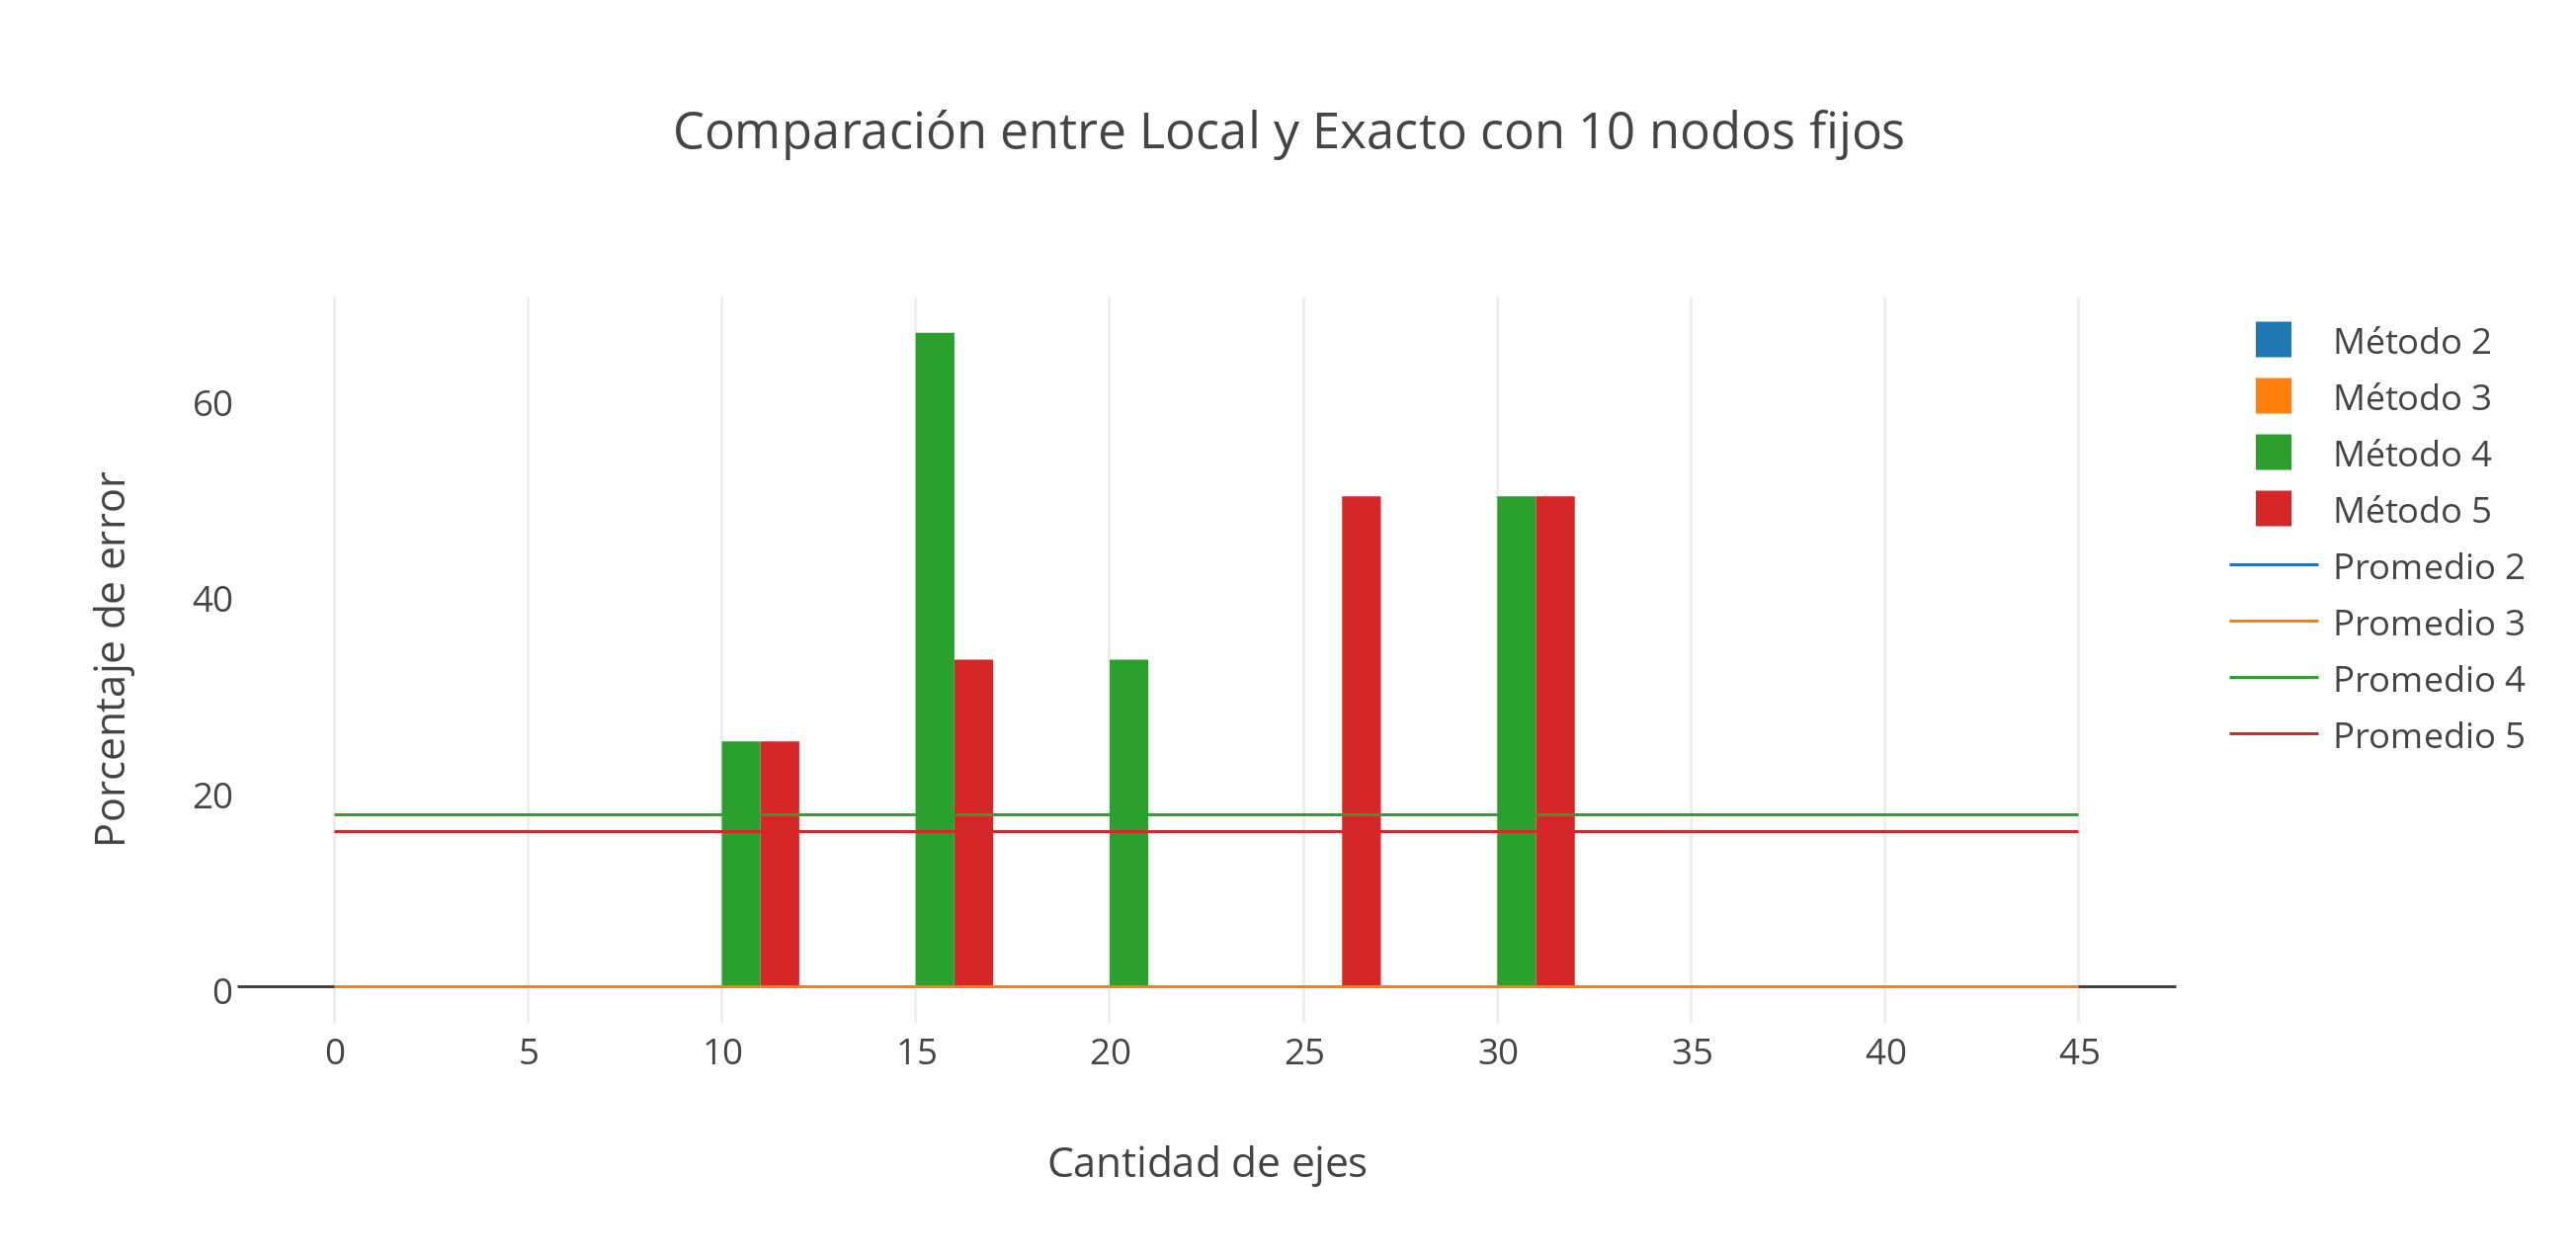
\includegraphics[scale=0.75]{imagenes/local/exacto/10nodos.png}
% 	\caption{}
%	\label{10Nodos}
   \end{center}
 \end{figure}

  \begin{figure}[h!]
   \begin{center}
 	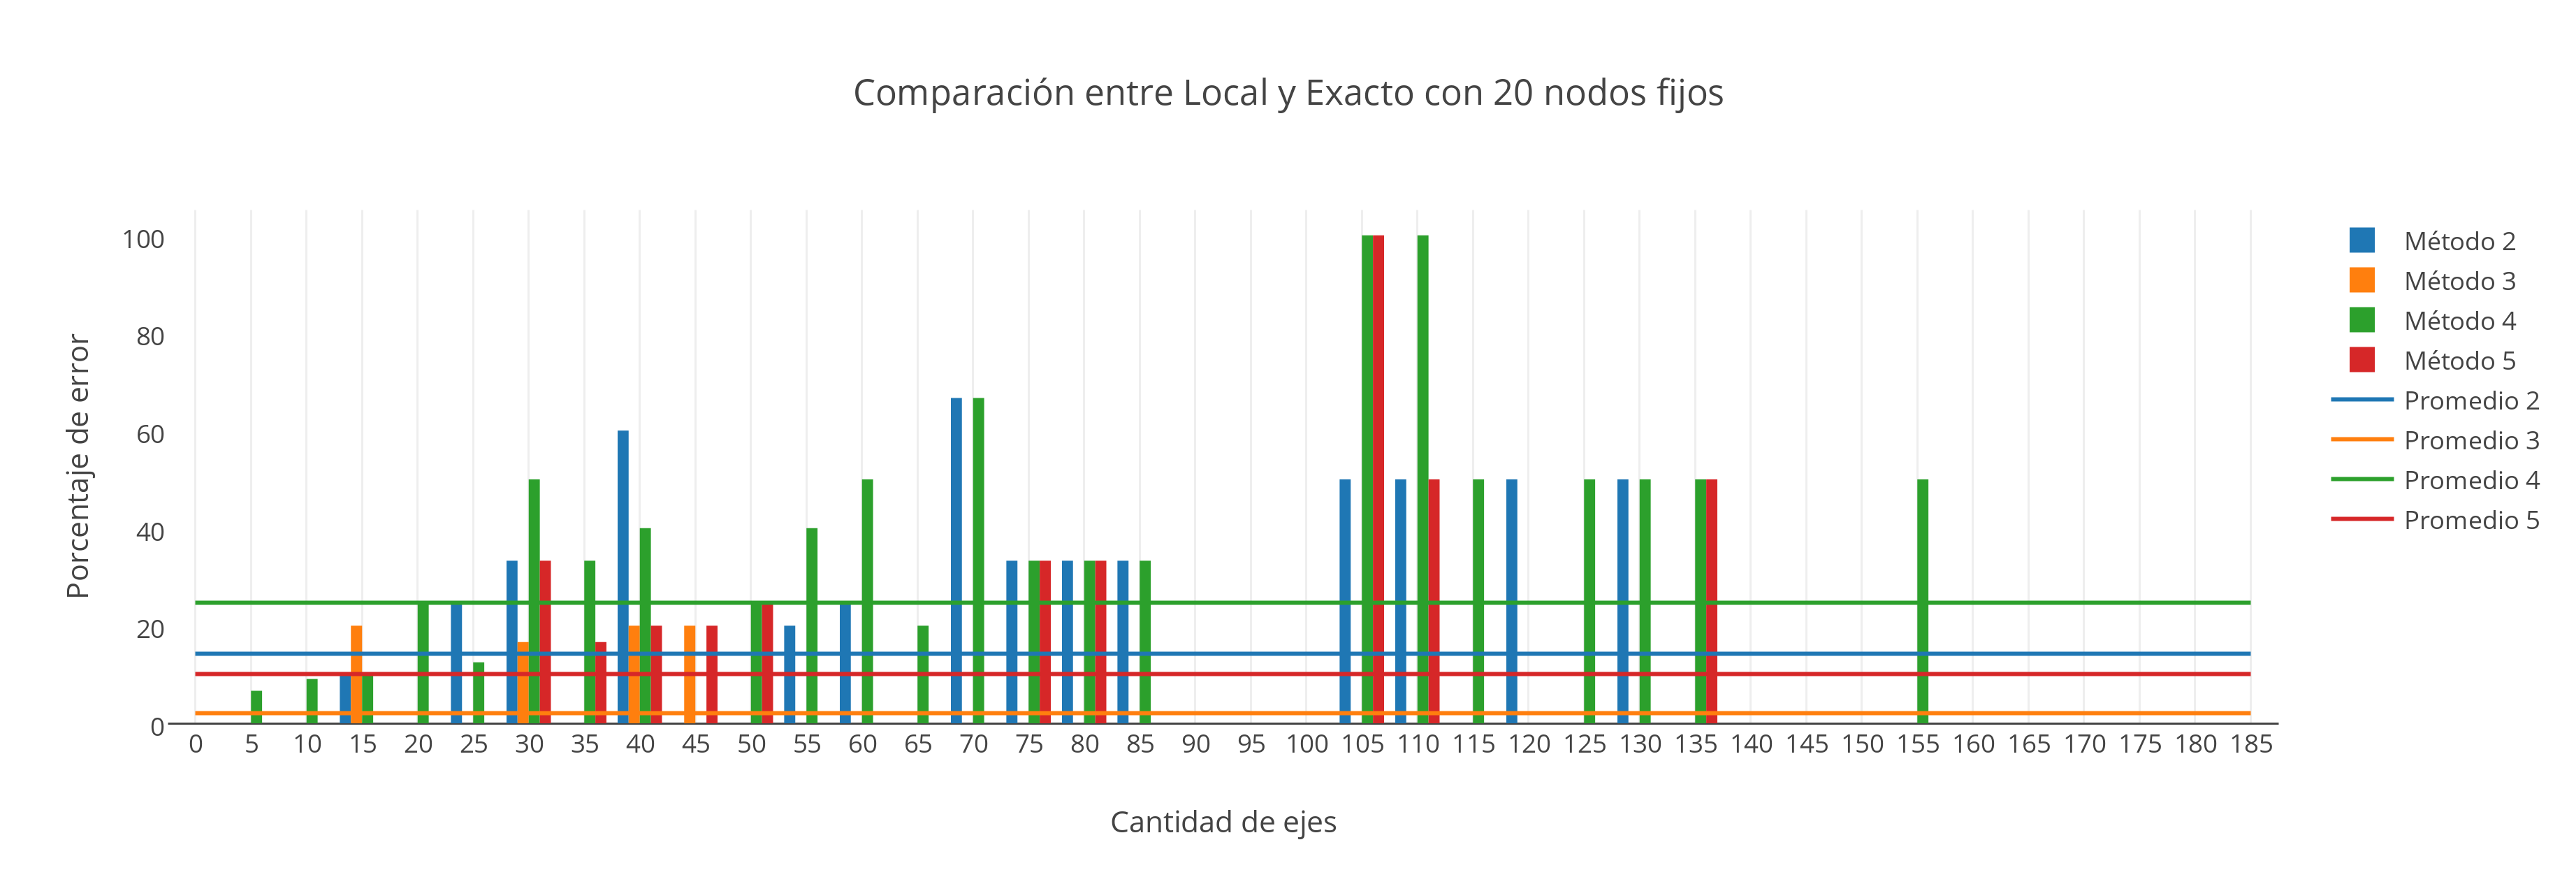
\includegraphics[scale=0.55]{imagenes/local/exacto/20nodos.png}
% 	\caption{}
%	\label{10Nodos}
   \end{center}
 \end{figure}
 
   \begin{figure}[h!]
   \begin{center}
 	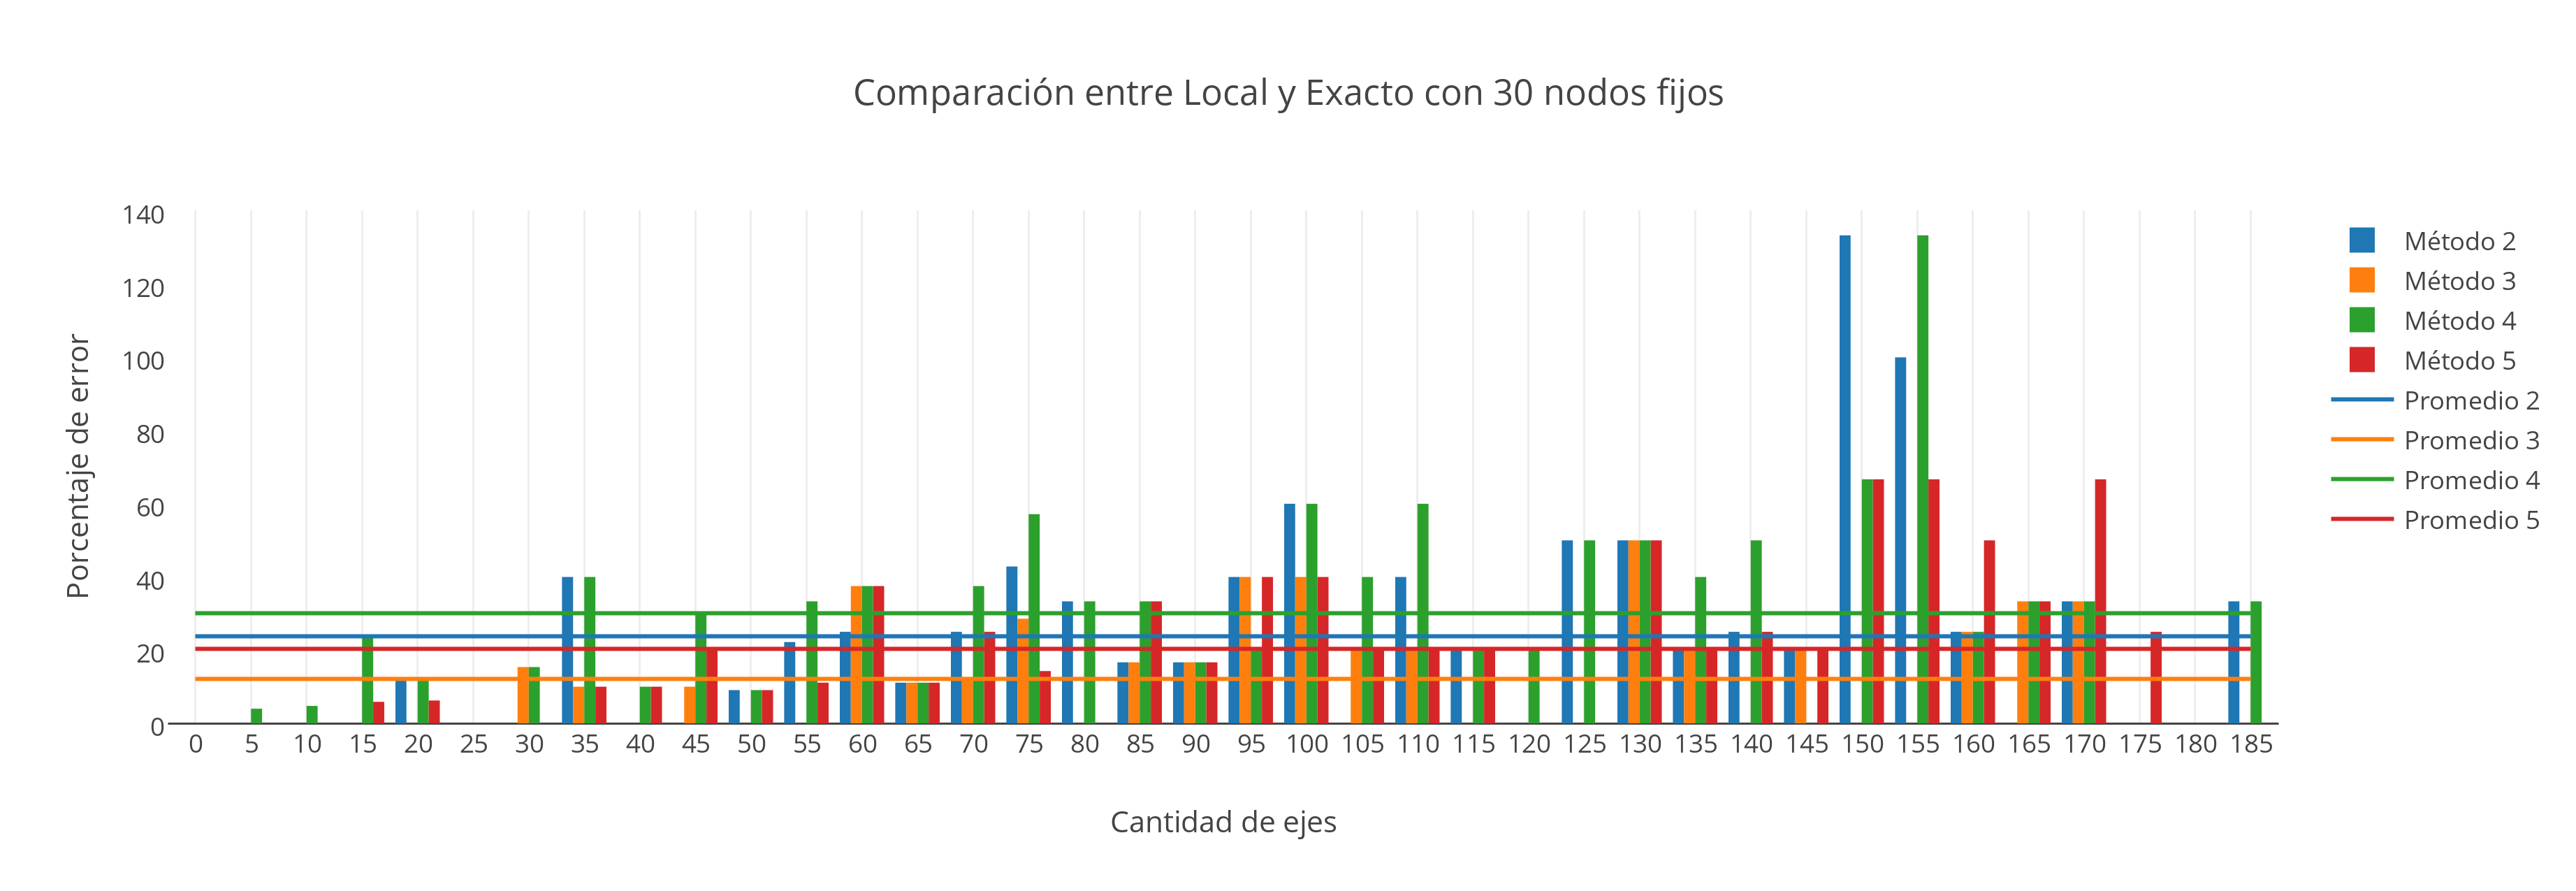
\includegraphics[scale=0.55]{imagenes/local/exacto/30nodos.png}
% 	\caption{}
%	\label{10Nodos}
   \end{center}
 \end{figure}

\newpage

  \begin{figure}[h!]
   \begin{center}
 	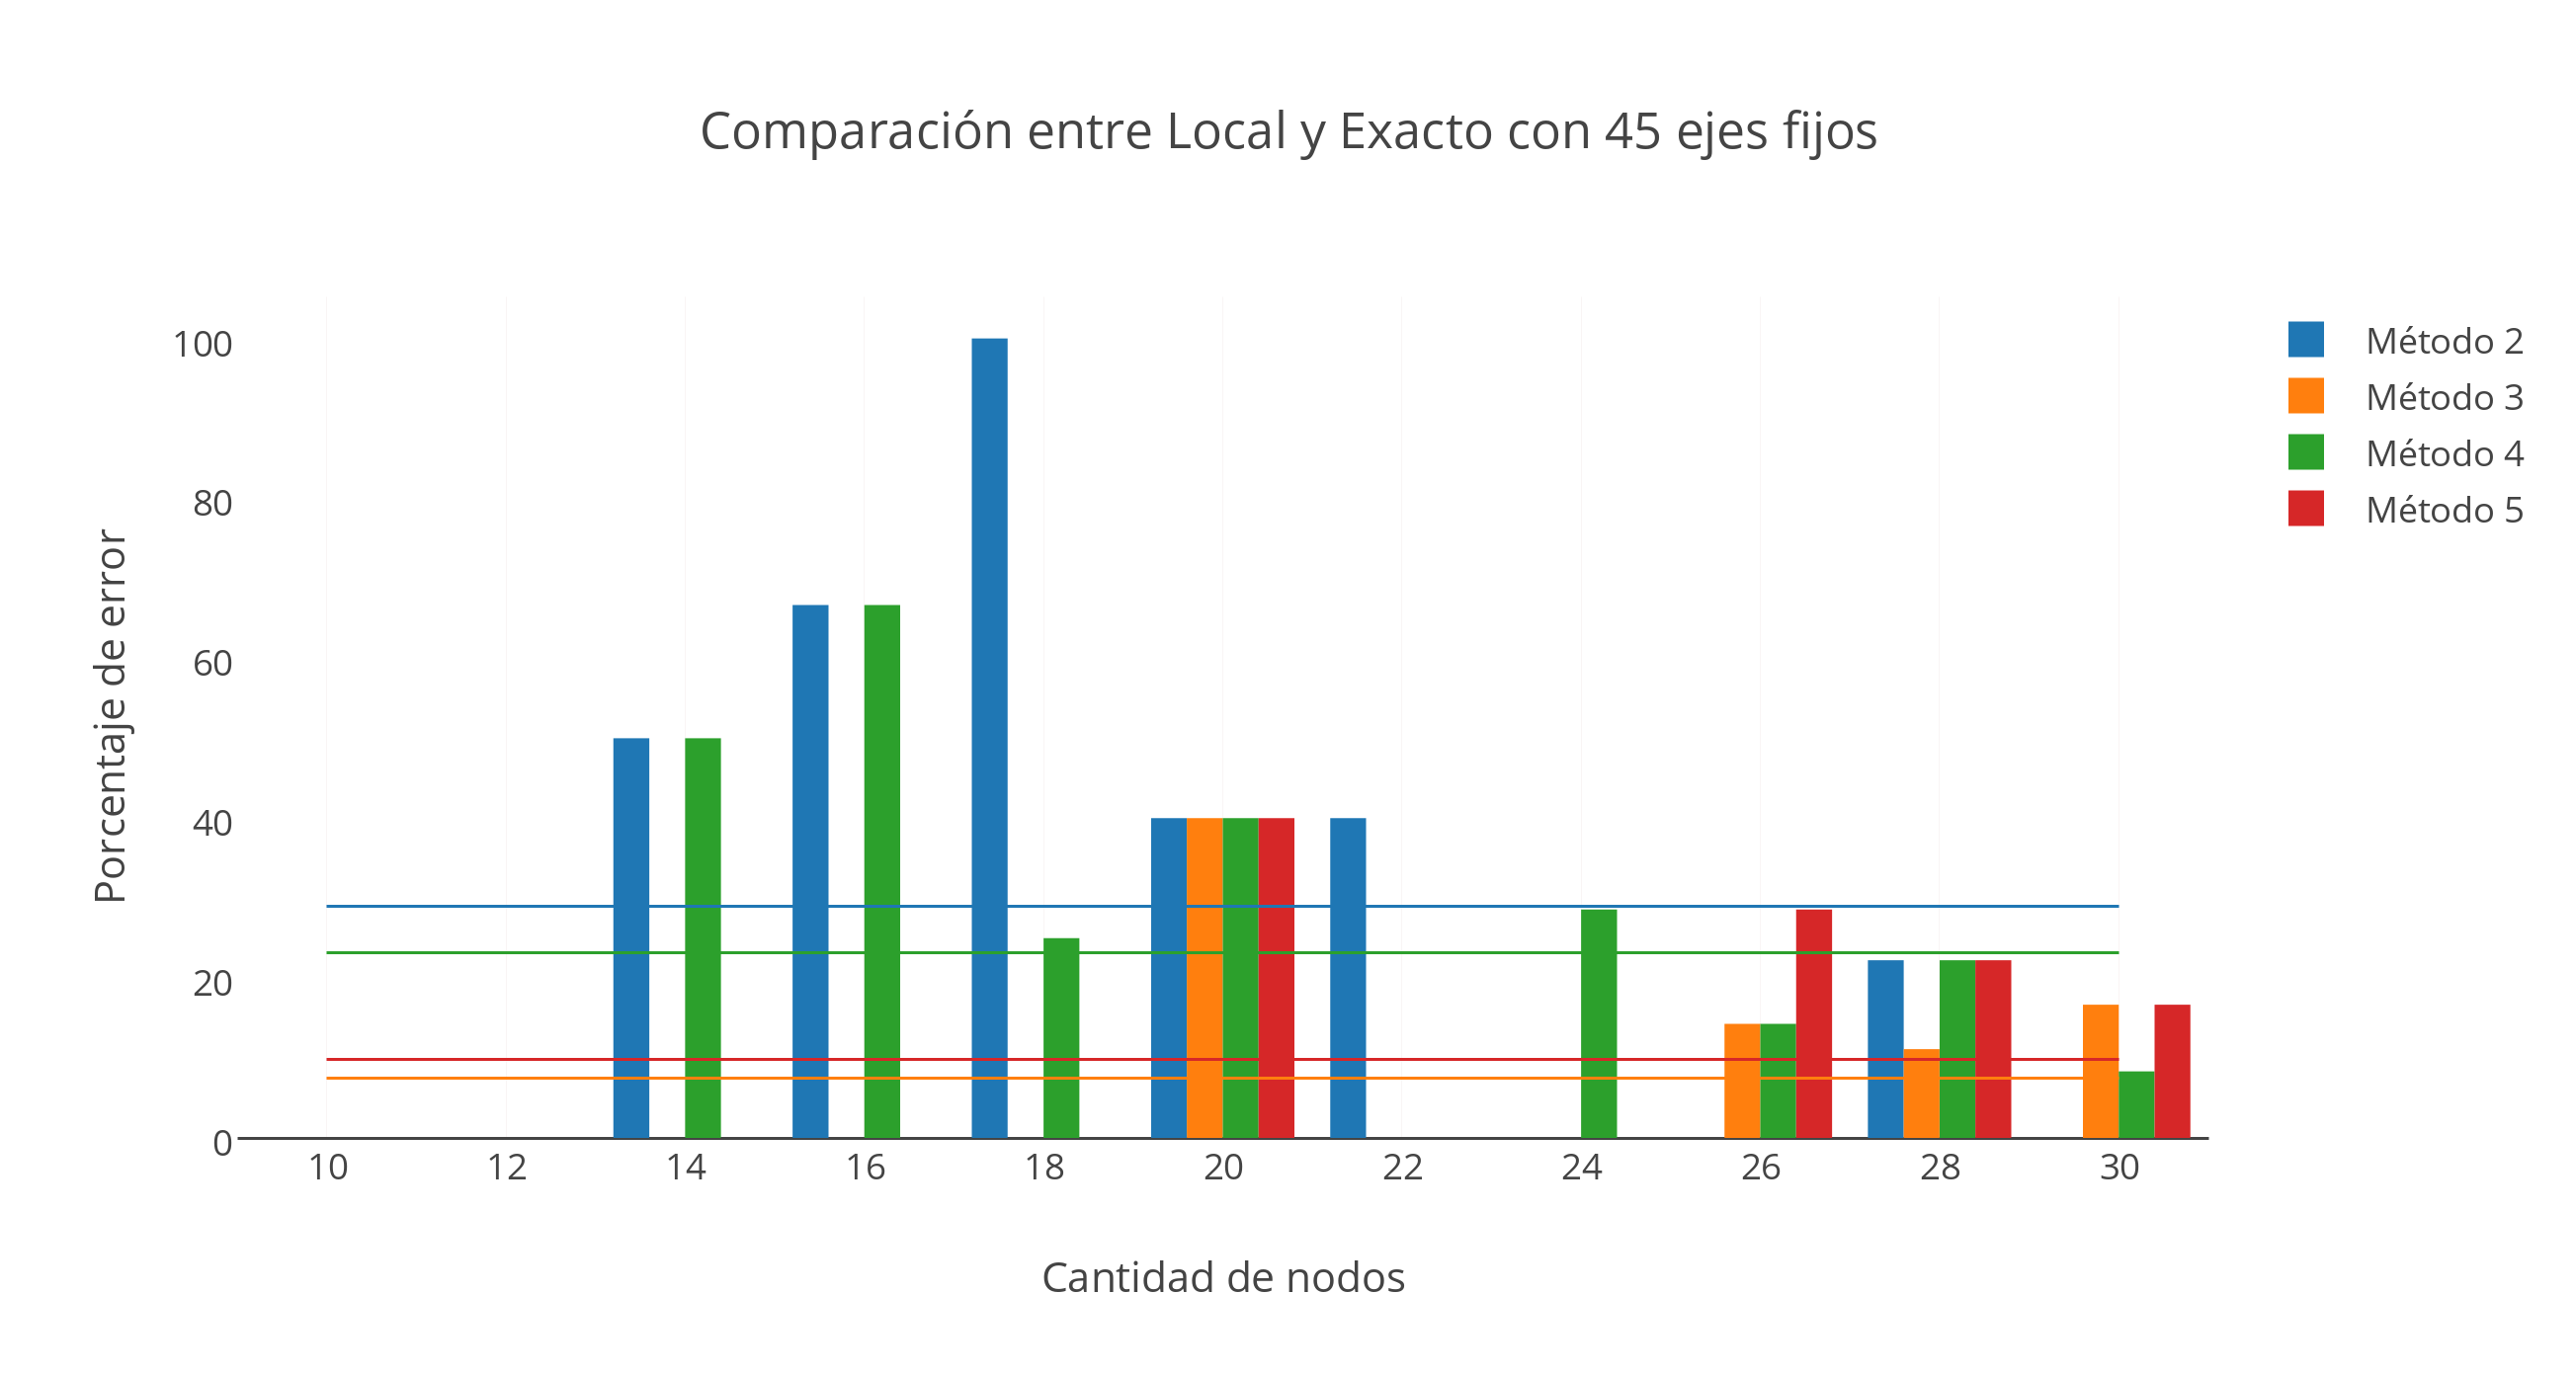
\includegraphics[scale=0.7]{imagenes/local/exacto/45ejes.png}
% 	\caption{}
%	\label{10Nodos}
   \end{center}
 \end{figure} 
 
  \begin{figure}[h!]
   \begin{center}
 	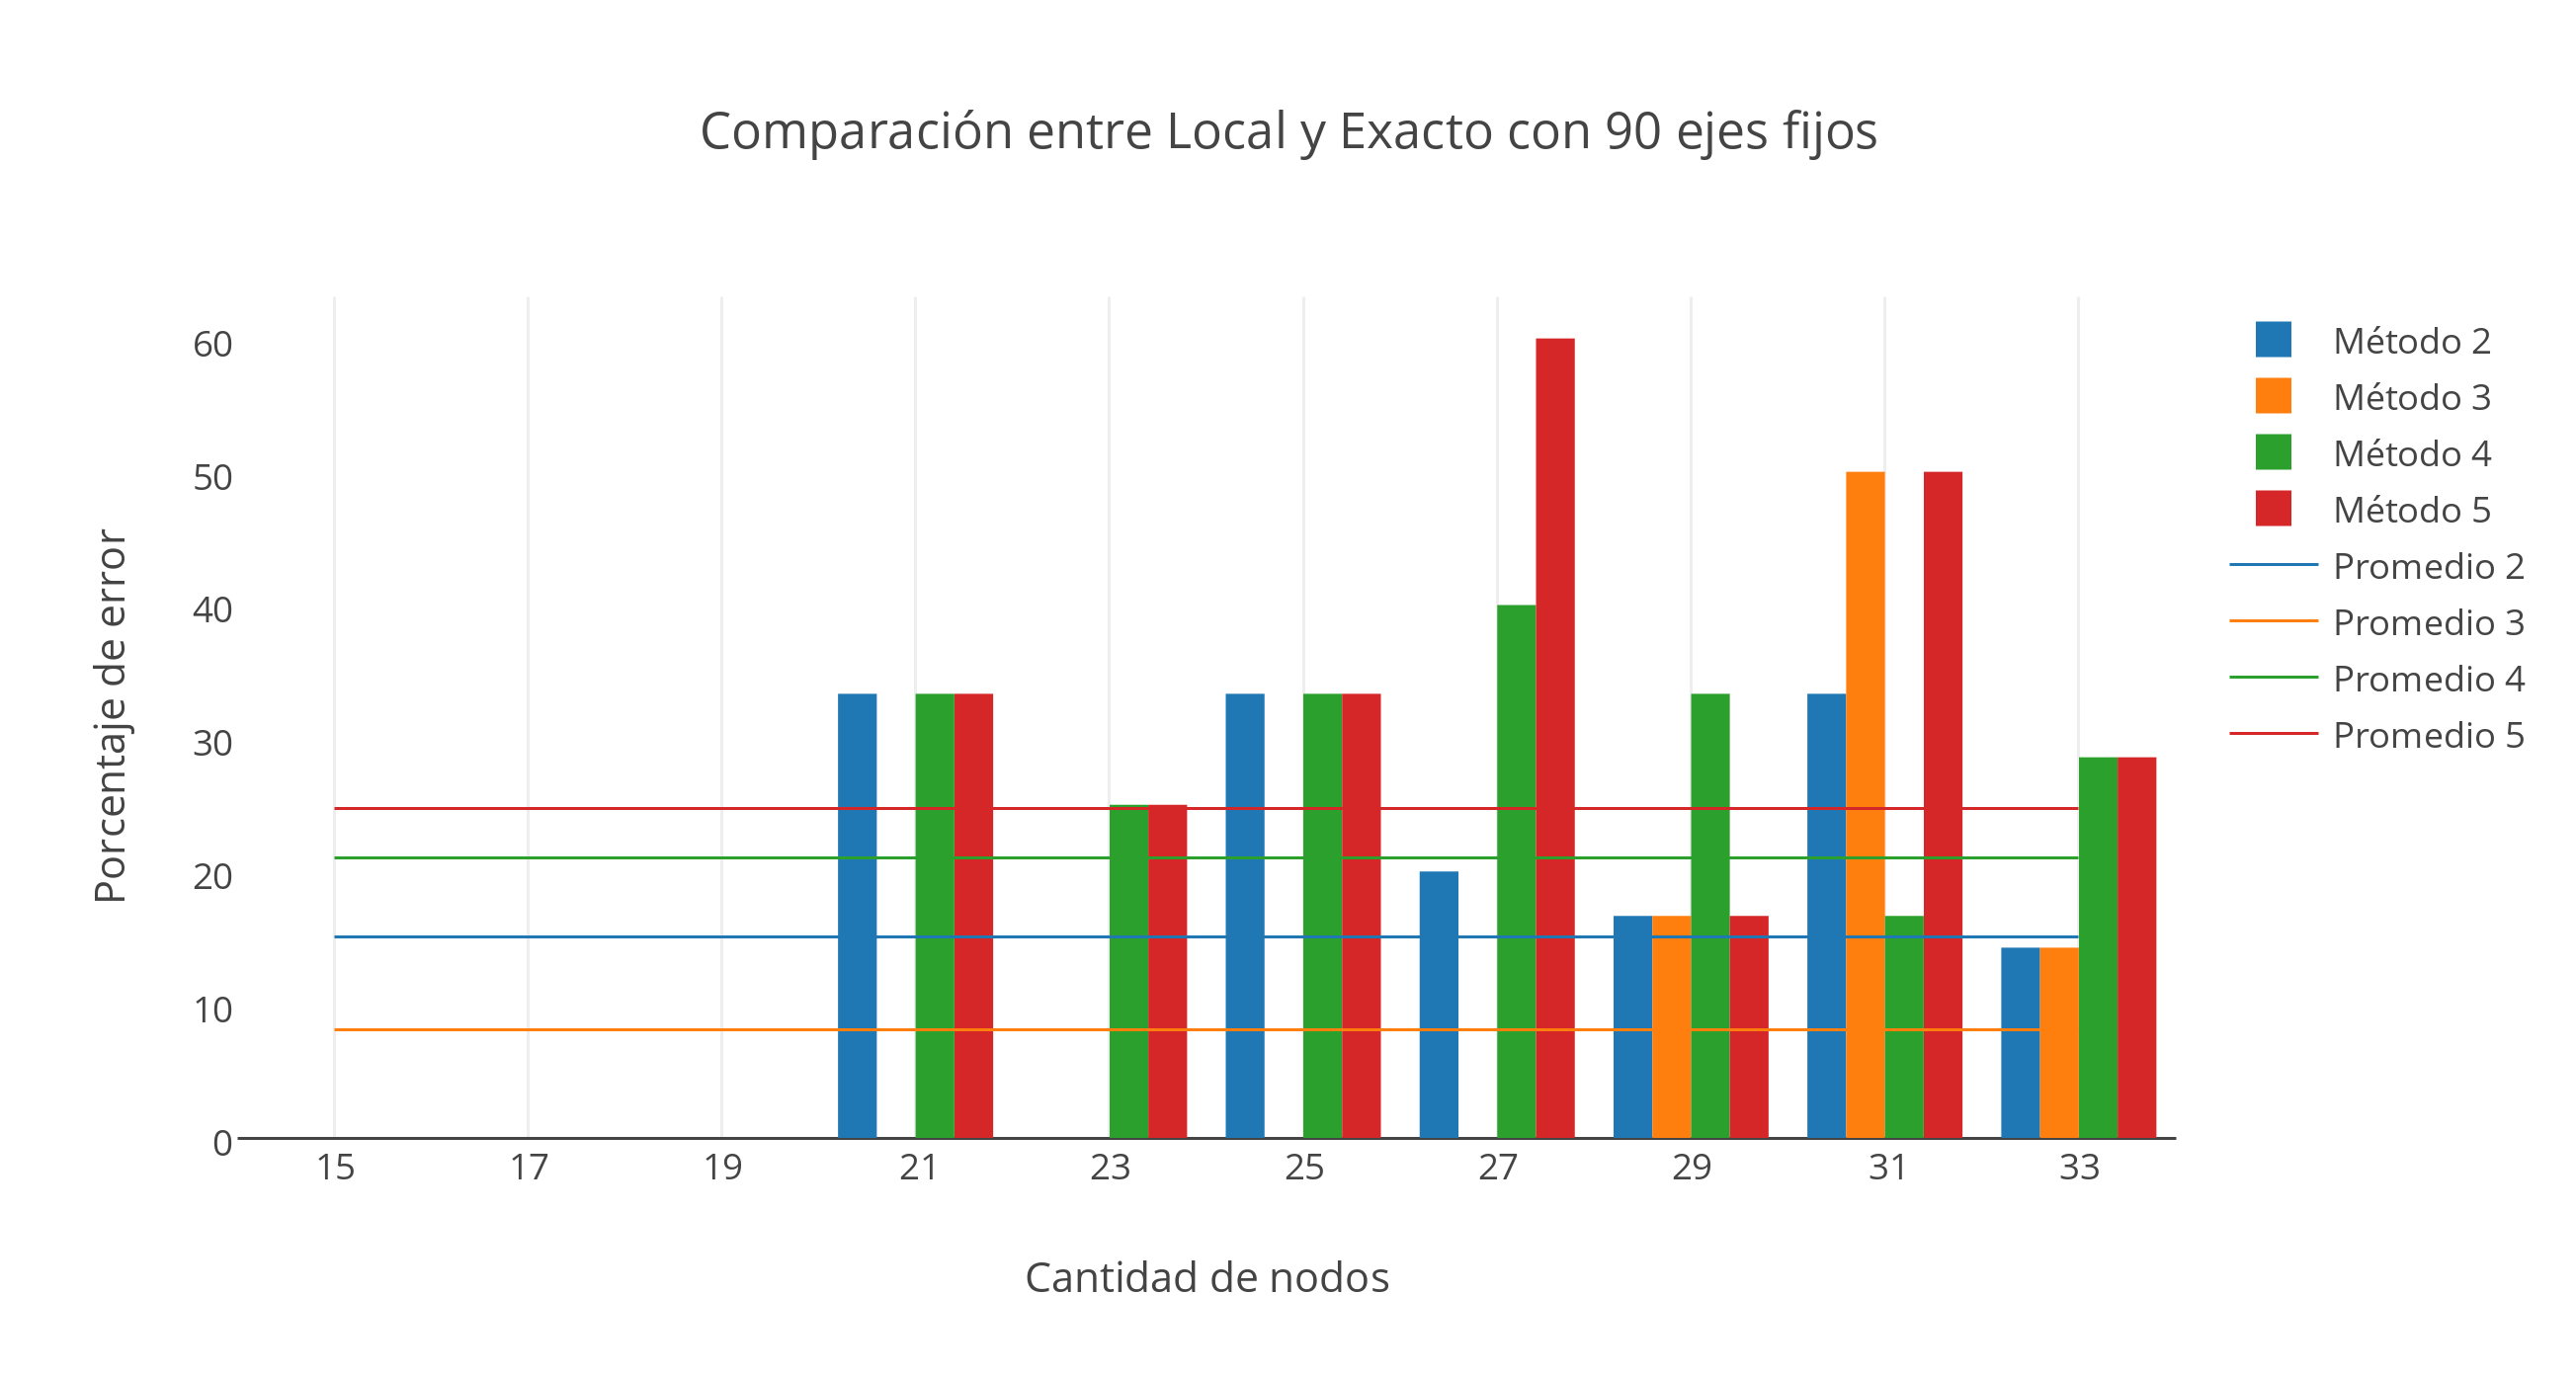
\includegraphics[scale=0.7]{imagenes/local/exacto/90ejes.png}
% 	\caption{}
%	\label{10Nodos}
   \end{center}
 \end{figure} 
 
  \begin{figure}[h!]
   \begin{center}
 	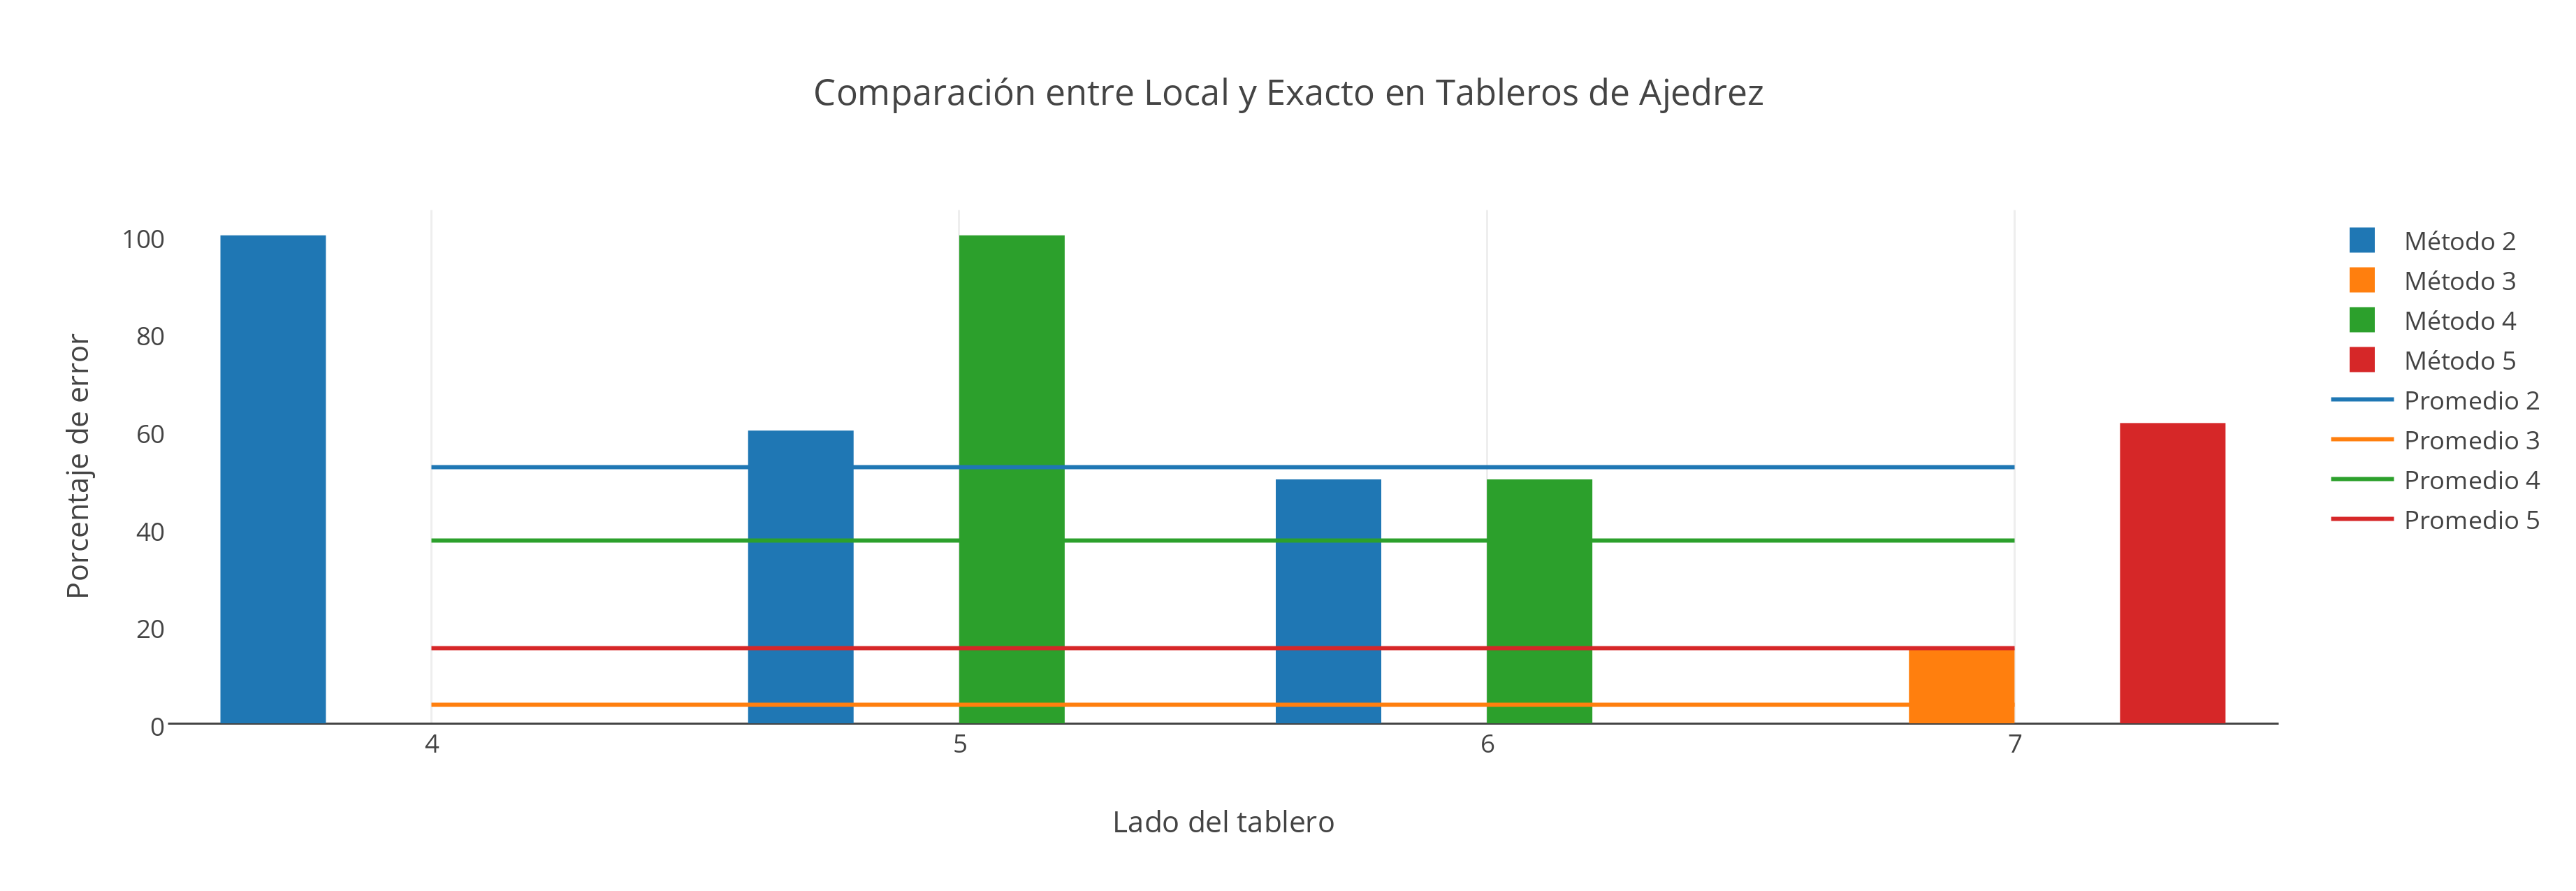
\includegraphics[scale=0.55]{imagenes/local/exacto/tableros.png}
% 	\caption{}
%	\label{10Nodos}
   \end{center}
 \end{figure} 
 
\newpage 
 
\subsubsection{Elecci\'on de versi\'on \'optima}

\newpage